\documentclass{beamer}
\usepackage{boondox-calo} % lowercase calligraphic letters
\usepackage[backend=biber]{biblatex}
\usepackage{optidef}

\beamertemplatenavigationsymbolsempty
\usetheme{Warsaw}
\addbibresource{reference.bib}
\setbeamertemplate{bibliography item}{\insertbiblabel}

%% label
% eq=equation
% pb=problem
% po=problem objective
% pc=problem constraint

%% miscellaneous
\renewcommand
{\th}
{\textsuperscript{th}}

%% math
\newcommand
{\voltage}
{V}

\newcommand
{\uniform}
[2]
{Uniform(#1, #2)}

\newcommand
{\transpose}
{^{\intercal}}

\newcommand
{\set}
[1]
{\left\{ #1 \right\}}

\newcommand
{\largeSetCondition}
{\middle|}

\newcommand
{\const}
{\mathfrak}

\renewcommand
{\vec}
[1]
{\boldsymbol{\mathbf{#1}}}

\newcommand
{\real}
{\mathbb{R}}

\newcommand
{\realNonneg}
[1]
{\real_{ + }^{ #1 }}

\newcommand
{\integerNonneg}
{\mathbb{Z}_{ + }}

\newcommand
{\unit}
[1]
{\left[ #1 \right]}

\DeclareMathOperator*{\argmax}{arg\,max}

\newcommand
{\gradient}
[2]
{\nabla_{#1}(#2)}

\newcommand
{\otherwise}
{\text{otherwise}}

\newcommand
{\inner}
[2]
{\langle #1, #2 \rangle}

%% problem
\newcommand
{\bsX}
{\const{x}}

\newcommand
{\bsY}
{\const{y}}

\newcommand
{\bsZ}
{\const{z}}

\newcommand
{\posMin}
{0}

\newcommand
{\posMax}
{1000}

\newcommand
{\constraintOne}
{
\addConstraint
  { \sum_{ \urllcUser }{ \urllcOldFour{\urllcUser}{\curTimeSlot}{\curTimeMinislot}{\subchannel} } }
  { \leq 1,\quad }
  { \forall\subchannel }
}

\newcommand
{\constraintTwo}
{
\addConstraint
  { \sum_{ \subchannel }{ \urllcOldFour{\urllcUser}{\curTimeSlot}{\curTimeMinislot}{\subchannel} } }
  { = \demandSubchannel{\urllcUser}{\curTimeSlot}{\curTimeMinislot},\quad }
  { \forall\urllcUser }
}

\newcommand
{\concaveBinaryFunc}
{g^{\prime}}

\newcommand
{\concaveBinary}
[1]
{\concaveBinaryFunc(#1)}

\newcommand
{\binaryFunc}
{\urllcOldFour{\urllcUser}{\curTimeSlot}{\curTimeMinislot}{\subchannel} \left( 1 - \urllcOldFour{\urllcUser}{\curTimeSlot}{\curTimeMinislot}{\subchannel} \right)}

\newcommand
{\feaSol}
[2]
{\urllcRa_{#1, #2}^{fs}}

\newcommand
{\feaSolVec}
{\urllcVec^{fs}}

\newcommand
{\penaltyMultiplier}
{\xi}

\newcommand
{\polyhedron}
{\mathcal{P}}

\newcommand
{\signal}
{q}

\newcommand
{\pulse}
[4]
{\signal(#1, #2, #3, #4)}

\newcommand
{\subcarrierSignal}
[3]
{\const{\signal}_{#1, #2}(#3)}

\newcommand
{\channelSignal}
[2]
{\const{\signal}_{#1}(#2)}

\newcommand
{\spec} % 3GPP specifications
[1]
{\textcolor{blue}{#1}}

\newcommand
{\bit}
{b}

\newcommand
{\encodeBit}
[2]
{\const{\bit}_{#1, #2}}

\newcommand
{\decodeBit}
[2]
{\bit_{#1, #2}}

\newcommand
{\phaseShift}
[1]
{\theta(#1)}

\newcommand
{\cof} % coefficient
[2]
{c_{#1, #2}}

\newcommand
{\subcarrier}
{e}

\newcommand
{\numerology}
{\mu}

\newcommand
{\power}
{p}

\newcommand
{\txPow}
{\const{\power}^{tx}}

\newcommand
{\freque}
{f}

\newcommand
{\frequency}
{\const{\freque}}

\newcommand
{\freq}
[1]
{\frequency_{#1}}

\newcommand
{\subcarrierFreq}
[1]
{\frequency_{#1}}

\newcommand
{\subcarrierSpacing}
{\zeta}

\newcommand
{\genericSubchannel}
{sc}

\newcommand
{\bandwidth}
{\const{w}}

\newcommand
{\subchannelBandwidth}
{\bandwidth^{\genericSubchannel}}

\newcommand
{\channelBandwidth}
{\bandwidth^{cn}}

\newcommand
{\guardBandwidth}
{\bandwidth^{gd}}

\newcommand
{\lightSpeed}
{3 \cdot 10^{8}}

\newcommand
{\distance}
{d}

\newcommand
{\pathLossExponent}
{\epsilon^{pl}}

\newcommand
{\shadowingStddv} % shadowing standard deviation
{\sigma^{sd}}

\newcommand
{\thermalNoiseDensity}
{\const{o}}

\newcommand
{\subchannelThermalNoise}
{\thermalNoiseDensity^{\genericSubchannel}}

\newcommand
{\utilFunc}
{g}

\newcommand
{\utilComp} % utility composite function
[1]
{\ln{#1}}

\newcommand
{\rate}
{r}

\newcommand
{\rateVec}
{\vec{\rate}}

\newcommand
{\peakRate}
{\const{\rate}}

\newcommand
{\avgRate} % average rate
[1]
{\bar{\rate}_{#1}}

\newcommand
{\relaxAvgRate}
[1]
{\bar{\rate}_{#1}^{\prime}}

\newcommand
{\weight}
{\epsilon}

\renewcommand
{\time}
{t}

\newcommand
{\timeDuration}
{\const{\time}}

\newcommand
{\chunkDuration}
{\timeDuration^{ck}}

\newcommand
{\symbolDuration}
{\timeDuration^{sb}}

\renewcommand
{\symbol}
{y}

\newcommand
{\curSymbol}
{\symbol_{0}}

\newcommand
{\cyclicPrefixDuration}
{\timeDuration^{cp}}

\newcommand
{\timeSlotDuration}
{\timeDuration^{sl}}

\newcommand
{\timeMinislotDuration}
{\timeDuration^{ms}}

\newcommand
{\timeSlot}
{n}

\newcommand
{\curTimeSlot}
{\timeSlot_{0}}

\newcommand
{\timeSlotNum}
{\const{\timeSlot}}

\newcommand
{\timeMinislot}
{m}

\newcommand
{\curTimeMinislot}
{\timeMinislot_{0}}

\newcommand
{\timeMinislotNum}
{\const{\timeMinislot}}

\newcommand
{\subchannel}
{l}

\newcommand
{\subchannelNum}
{\const{\subchannel}}

\newcommand
{\superposition}
{\sum_{ \subcarrier = 0 }^{ 611 }{ 5 \cos( 2 \pi \subcarrierSpacing \subcarrier \time + \phaseShift{\encodeBit{\subcarrier}{\curSymbol}} ) }}

%% embb macro
\newcommand
{\embbUser}
{u}

\newcommand
{\embbUserNum}
{\const{\embbUser}}

\newcommand
{\embbRa} % embb resource allocation
{\alpha}

\newcommand
{\embbVec} % embb vector
{\vec{\embbRa}}

\newcommand
{\relaxEmbbVec}
{\embbVec^{\prime}}

\newcommand
{\curEmbbVec}
[1]
{\embbVec_{#1}}

\newcommand
{\relaxCurEmbbVec}
[1]
{\curEmbbVec{#1}^{\prime}}

\newcommand
{\relaxCurEmbbVecOpt}
[1]
{\curEmbbVec{#1}^{\prime \ast}}

\newcommand
{\movModAvgRate} % moving modified average rate
[3]
{\tilde{\modRate}_{#1, #2, #3}}

\newcommand
{\movAvgRate}
{\tilde{\rate}}

\newcommand
{\movAvgRateVec}
[1]
{\vec{\movAvgRate}_{#1}^{\prime}}

\newcommand
{\movAvgRateMinislot}
[2]
{\tilde{\psi}_{#1, #2}}

\newcommand
{\relaxMovAvgRateTwo}
[2]
{\movAvgRate_{#1, #2}^{\prime}}

\newcommand
{\embbThree}
[3]
{\embbRa_{#1, #2, #3}}

\newcommand
{\relaxEmbbThree}
[3]
{\embbRa_{#1, #2, #3}^{\prime}}

\newcommand
{\rateSlotOne}
[1]
{\rate_{#1}}

\newcommand
{\rateSlotTwo}
[2]
{\rate_{#1, #2}}

\newcommand
{\relaxRateSlotTwo}
[2]
{\rateSlotTwo{#1}{#2}^{\prime}}

\newcommand
{\relaxRateSlotTwoOpt}
[2]
{\rateSlotTwo{#1}{#2}^{\prime \ast}}

\newcommand
{\pRateSlot}
[3]
{\peakRate_{#1, #2, #3}}

\newcommand
{\relaxCurRateSlotVec}
[1]
{\rateVec_{#1}^{\prime}}

\newcommand
{\embbDist}
[2]
{\const{\distance}_{#1, #2}}

\newcommand
{\pls} % path loss and shadowing
{h}

\newcommand
{\plsFunc}
[2]
{\pls(#1, #2)}

\newcommand
{\embbPls}
[3]
{\const{\pls}_{#1, #2, #3}}

\newcommand
{\embbPow}
[3]
{\const{\power}_{#1, #2, #3}}

\newcommand
{\embbMat}
[2]
{A_{#1, #2}}

\newcommand
{\embbX}
[2]
{X_{#1, #2}}

\newcommand
{\embbY}
[2]
{Y_{#1, #2}}

\newcommand
{\embbZ}
[2]
{\const{z}_{#1, #2}}

%% urllc macro
\newcommand
{\urllcUser}
{v}

\newcommand
{\urllcUserNum}
{\const{\urllcUser}}

\newcommand
{\urllcRa} % urllc resource allocation
{\beta}

\newcommand
{\urllcVec} % urllc vector
{\vec{\urllcRa}}

\newcommand
{\curUrllcVec}
[2]
{\urllcVec_{#1, #2}}

\newcommand
{\urllcFive}
[5]
{\urllcRa_{#1, #2, #3, #4, #5}}

\newcommand
{\urllcOldFour}
[4]
{\urllcRa_{#1, #2, #3, #4}}

\newcommand
{\rateMinislot}
[3]
{\rate_{#1, #2, #3}}

\newcommand
{\modRate}
{\phi}

\newcommand
{\modRateMinislot}
[3]
{\modRate_{#1, #2, #3}}

\newcommand
{\modPeakRateMinislot}
[3]
{\varphi_{#1, #2, #3}}

\newcommand
{\demandRate}
{R}

\newcommand
{\dRateThree}
[3]
{\demandRate_{#1, #2, #3}}

\newcommand
{\pRateMinislot}
[4]
{\peakRate_{#1, #2, #3, #4}}

\newcommand
{\pRateMinislotMin}
[3]
{\peakRate_{#1, #2, #3}^{\genericSubchannel}}

\newcommand
{\urllcDist}
[3]
{\const{\distance}_{#1, #2, #3}}

\newcommand
{\urllcPls}
[4]
{\const{\pls}_{#1, #2, #3, #4}}

\newcommand
{\urllcPow}
[4]
{\const{\power}_{#1, #2, #3, #4}}

\newcommand
{\urllcMat}
[2]
{B_{#1, #2}}

\newcommand
{\demandSubchannel}
[3]
{D_{#1, #2, #3}}

\newcommand
{\urllcX}
[3]
{X_{#1, #2, #3}}

\newcommand
{\urllcY}
[3]
{Y_{#1, #2, #3}}

\newcommand
{\urllcZ}
[3]
{\const{z}_{#1, #2, #3}}

\title{Multiplexing URLLC Traffic Within eMBB Services in 5G NR: Fair Scheduling}
\author{Hao Yin, Lyutianyang Zhang, Sumit Roy}
\institute{Department of Electrical and Computer Engineering, University of Washington, Seattle, USA}
\date{February, 2021}

\begin{document}

\begin{frame}
  \titlepage
  Published in IEEE Transactions on Communications
\end{frame}

\section{System Model}
\begin{frame}
  \frametitle{System Model}
  \begin{itemize}
    \item One base station, downlink transmission, OFDMA, eMBB and URLLC users.
    \item Saturated eMBB traffic \cite{S05}: Each eMBB user has infinite amount of data to be served.
  \end{itemize}
  \begin{figure}
    \includegraphics[width=0.6\textwidth]{system_model}
    \caption{System model}
  \end{figure}
\end{frame}

\subsection{Parameters}
\begin{frame}
  \frametitle{Parameters}
  \begin{itemize}
    \item Base frequency (use only when discuss channel model and do simulation, otherwise \textcolor{red}{assume $0$ for simplicity})
      \begin{equation*}
        \freq{0} = 28 \unit{GHz}
      \end{equation*}
    \item Number of time slots
      \begin{equation}
        \timeSlotNum = 200
      \end{equation}
   \item Number of time minislots per time slot
      \begin{equation*}
        \timeMinislotNum = 7
      \end{equation*}
  \end{itemize}
\end{frame}

\begin{frame}
  \begin{itemize}
    \item Position of base station
      \begin{align}
        \bsX &= 500 &\unit{m}\\
        \bsY &= 500 &\unit{m}\\
        \bsZ &= 100 &\unit{m}
      \end{align}
  \end{itemize}
\end{frame}

\begin{frame}
  \begin{itemize}
    \item Number of eMBB users
      \begin{equation}
        \embbUserNum = 100
      \end{equation}
    \item Begin position of eMBB users
      \begin{align}
        \embbX{\embbUser}{0} &\sim \uniform{\posMin}{\posMax} &\unit{m},\quad \forall\embbUser\\
        \embbY{\embbUser}{0} &\sim \uniform{\posMin}{\posMax} &\unit{m},\quad \forall\embbUser\\
        \embbZ{\embbUser}{0} &= 0 &\unit{m},\quad \forall\embbUser
      \end{align}
    \item End position of eMBB users
      \begin{align}
        \embbX{\embbUser}{\timeSlotNum - 1} &\sim \uniform{\posMin}{\posMax} &\unit{m}, \quad \forall\embbUser\\
        \embbY{\embbUser}{\timeSlotNum - 1} &\sim \uniform{\posMin}{\posMax} &\unit{m}, \quad \forall\embbUser\\
        \embbZ{\embbUser}{\timeSlotNum - 1} &= 0 &\unit{m},\quad \forall\embbUser
      \end{align}
  \end{itemize}
\end{frame}

\begin{frame}
  \begin{itemize}
    \item Number of URLLC users
      \begin{equation}
        \urllcUserNum = 10
      \end{equation}
    \item Begin position of URLLC users
      \begin{align}
        \urllcX{\urllcUser}{0}{0} &\sim \uniform{\posMin}{\posMax} &\unit{m},\quad \forall\urllcUser\\
        \urllcY{\urllcUser}{0}{0} &\sim \uniform{\posMin}{\posMax} &\unit{m},\quad \forall\urllcUser\\
        \urllcZ{\urllcUser}{0}{0} &= 0 &\unit{m},\quad \forall\urllcUser
      \end{align}
    \item End position of URLLC users
      \begin{align}
        \urllcX{\urllcUser}{\timeSlotNum - 1}{\timeMinislotNum - 1} &\sim \uniform{\posMin}{\posMax} &\unit{m}, \quad \forall\urllcUser\\
        \urllcY{\urllcUser}{\timeSlotNum - 1}{\timeMinislotNum - 1} &\sim \uniform{\posMin}{\posMax} &\unit{m}, \quad \forall\urllcUser\\
        \urllcZ{\urllcUser}{\timeSlotNum - 1}{\timeMinislotNum - 1} &= 0 &\unit{m},\quad \forall\urllcUser
      \end{align}
  \end{itemize}
\end{frame}

\begin{frame}
  \begin{itemize}
    \item URLLC demand
      \begin{equation}
        \dRateThree{\urllcUser}{\timeSlot}{\timeMinislot} \sim \uniform{0}{4000} \unit{\frac{ bits }{ minislot }},\quad \forall\urllcUser, \forall\timeSlot, \forall\timeMinislot
      \end{equation}
    \item URLLC demand peaks 500B per minislot, equivalently 14MBs.
  \end{itemize}
\end{frame}

\begin{frame}
  \begin{itemize}
    \item Channel bandwidth
      \begin{align*}
        \channelBandwidth &= 40 &\unit{MHz}\\
        &= 4 \cdot 10^{ 7 } &\unit{Hz}
      \end{align*}
    \item Numerology ($\numerology \in \set{ 0, 1 }$ is for Sub-6GHz)
      \begin{equation*}
        \numerology = 2
      \end{equation*}
    \item Number of subchannels
      \begin{equation*}
        \subchannelNum = 51
      \end{equation*}
   \end{itemize}
\end{frame}

\begin{frame}
  \begin{itemize}
    \item Transmission power
      \begin{align}
        \txPow &= 100 &\unit{W}\\
        &= 20 &\unit{dB}
      \end{align}
    \item Thermal noise density
      \begin{align}
        \thermalNoiseDensity &= -174 &\unit{\frac{ dBm }{ Hz }}\\
        &= -204 &\unit{\frac{ dB }{ Hz }}
      \end{align}
  \end{itemize}
\end{frame}

\subsection{Bandwidth}
\begin{frame}
  \frametitle{Bandwidth}
  \begin{itemize}
    \item Subcarrier spacing (SCS)
      \begin{align}
        \subcarrierSpacing &= 2^{ \numerology } \cdot \spec{15} &\unit{kHz}\\
        &= 60 &\unit{kHz}
      \end{align}
    \item Subchannel bandwidth
      \begin{align}
        \subchannelBandwidth &= \spec{12} \cdot \subcarrierSpacing &\unit{kHz}\\
        &= 2^{ \numerology } \cdot 180 &\unit{kHz}\\
        &= 720 &\unit{kHz}\\
        &= 7.2 \cdot 10^{ 5 } &\unit{Hz}
      \end{align}
  \end{itemize}
\end{frame}

\begin{frame}
  \begin{itemize}
    \item Guard bandwidth
      \begin{align}
        \guardBandwidth &= \frac{ \channelBandwidth - \subchannelNum \cdot \subchannelBandwidth }{ 2 } &\unit{Hz}\\
        &= 16.4 \cdot 10^{ 5 } &\unit{Hz}
      \end{align}
  \end{itemize}
\end{frame}

\begin{frame}
  \begin{figure}
    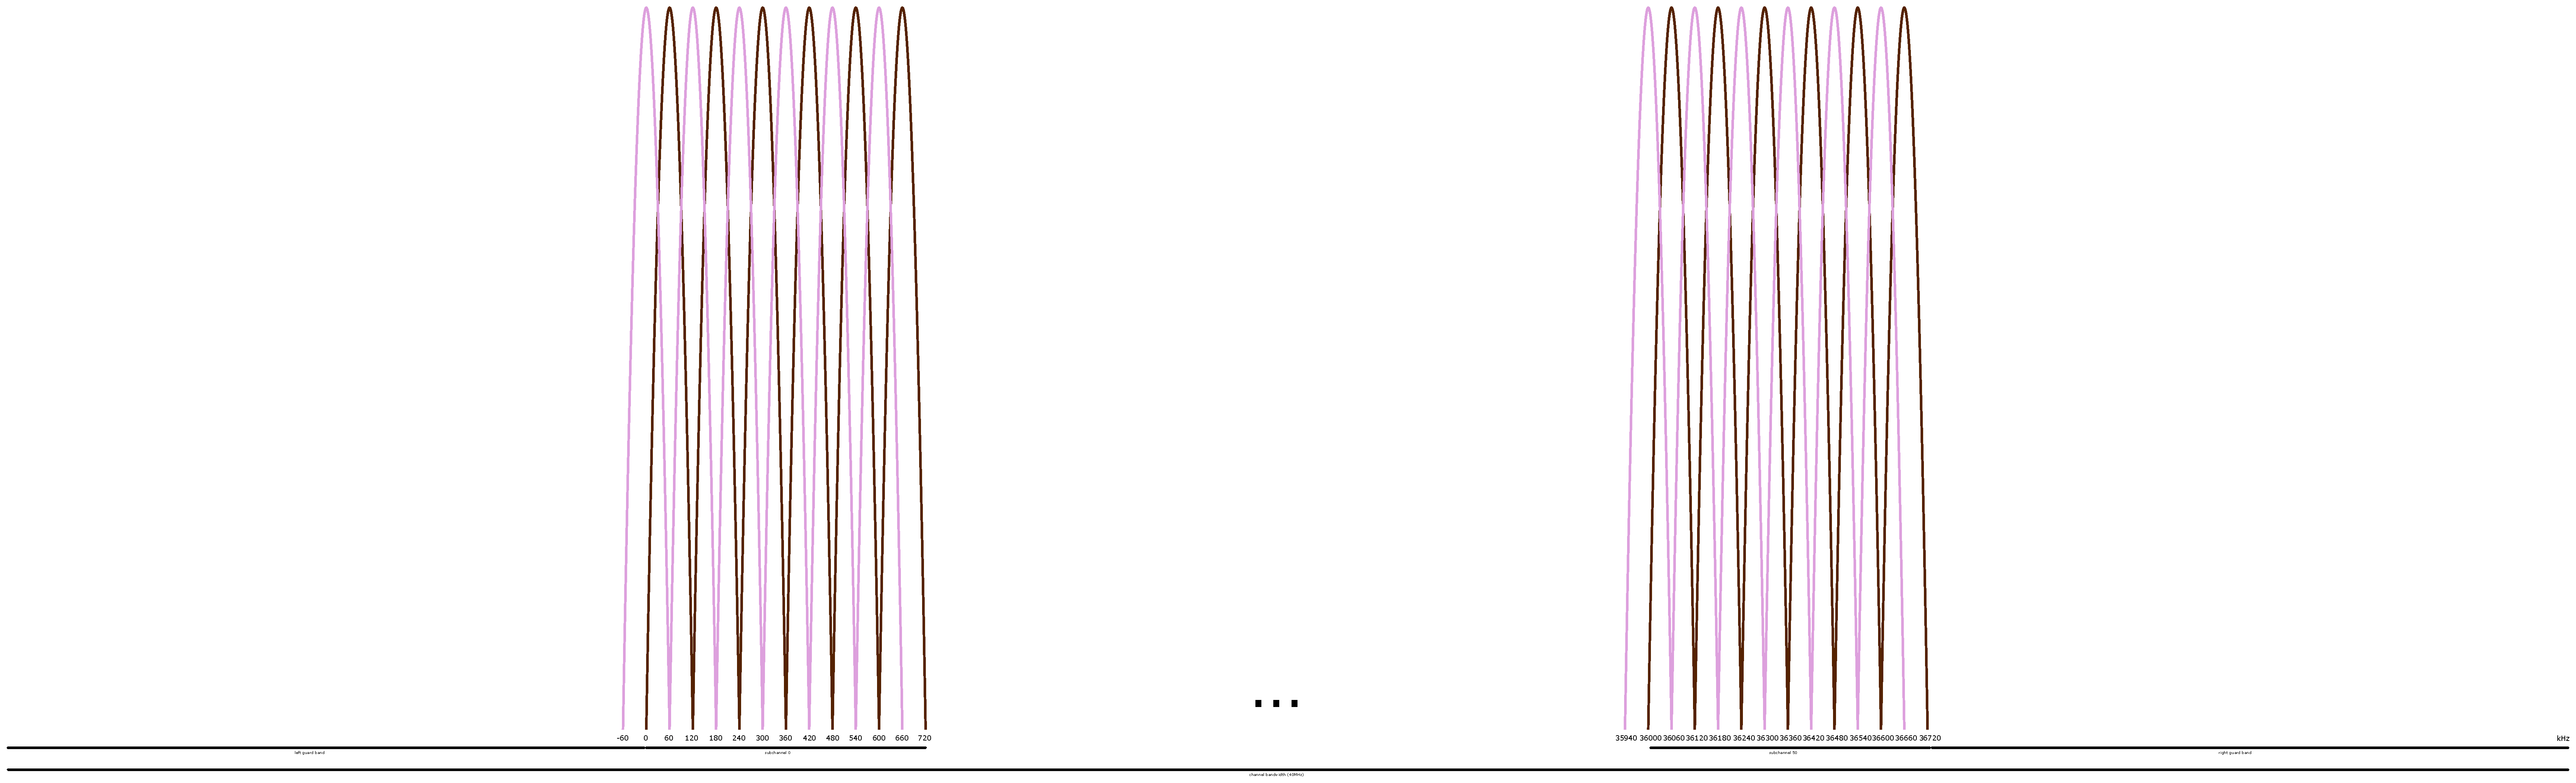
\includegraphics[width=\textwidth]{bandwidth}
    \caption{A Discrete Fourier Transform (DFT) coefficients example}
  \end{figure}
\end{frame}

\subsection{Duration}
\begin{frame}
  \frametitle{Duration}
  \begin{itemize}
    \item Time slot duration
      \begin{align}
        \timeSlotDuration &= \frac{ \spec{1} }{ 2^{ \numerology } } &\unit{ms}\\
        &= 0.25 &\unit{ms}\\
        &= 2.5 \cdot 10^{ -4 } &\unit{s}
      \end{align}
    \item Time minislot duration
      \begin{align}
        \timeMinislotDuration &= \frac{ \timeSlotDuration }{ \timeMinislotNum } &\unit{s}\\
        &= \frac{ 1 }{ 28 } \cdot 10^{ -3 } &\unit{s}
      \end{align}
  \end{itemize}
\end{frame}

\begin{frame}
  \begin{figure}
    \includegraphics[width=\textwidth]{duration}
    \caption{Duration}
  \end{figure}
\end{frame}

\subsection{Orthogonal Frequency-Division Multiple Access (OFDMA)}
\begin{frame}
  \frametitle{OFDMA}
  \begin{itemize}
    \item Chunk duration
      \begin{align}
        \chunkDuration &= \frac{ \timeSlotDuration }{ \spec{14} } &\unit{s}\\
        &= \frac{ 125 }{ 7 } \cdot 10^{ -6 } &\unit{s}
      \end{align}
    \item Symbol duration (enforced by DFT)
      \begin{align}
        \symbolDuration &= \frac{ 1 }{ \subcarrierSpacing } &\unit{ms}\\
        &= \frac{ 50 }{ 3 } \cdot 10^{ -6 } &\unit{s}
      \end{align}
  \end{itemize}
\end{frame}

\begin{frame}
  \begin{itemize}
    \item Cyclic prefix duration
      \begin{align}
        \cyclicPrefixDuration &= \chunkDuration - \symbolDuration &\unit{s}\\
        &= \frac{ 25 }{ 21 } \cdot 10^{ -6 } &\unit{s}
      \end{align}
  \end{itemize}
\end{frame}

\begin{frame}
  \begin{figure}
    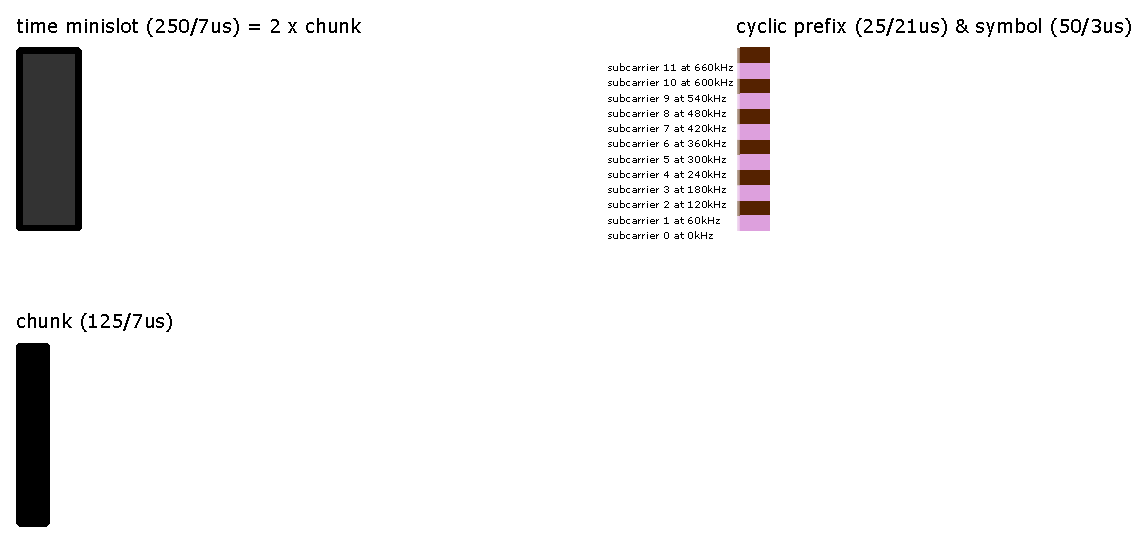
\includegraphics[width=\textwidth]{ofdma}
    \caption{OFDMA}
  \end{figure}
\end{frame}

\section{Orthogonal Frequency-Division Multiplexing (OFDM)}
\begin{frame}
  \frametitle{OFDM Analytical Concept}
  \begin{itemize}
    \item Assume no cyclic prefix for simplicity
      \begin{equation}
        \chunkDuration = \symbolDuration = \frac{ 1 }{ \subcarrierSpacing }
      \end{equation}
  \end{itemize}
\end{frame}

\subsection{Encoding}
\begin{frame}
  \frametitle{Encoding}
  \begin{itemize}
    \item Baseband modulation -- binary phase shift keying (BPSK)
      \begin{itemize}
        \item One symbol contains one bit
        \item Non-quadrature communication i.e. no complex numbers
      \end{itemize}
      \begin{equation}
        \phaseShift{\bit} =
        \begin{cases}
          0 &\bit = 0\\
          \pi &\bit = 1
        \end{cases} \unit{radians}
      \end{equation}
  \end{itemize}
\end{frame}

\begin{frame}
  \begin{itemize}
    \item Pulse
      \begin{equation}
        \pulse{\symbol}{\subcarrier}{\bit}{\time} =
        \begin{cases}
          5 \cos( 2 \pi \frac{ 1 }{ \symbolDuration } \subcarrier \time + \phaseShift{\bit} ) &\symbolDuration \symbol \leq \time < \symbolDuration \left( \symbol + 1 \right)\\
          0 &\otherwise
        \end{cases} \unit{\voltage}
      \end{equation}
    \item where $\symbol \in \integerNonneg, \subcarrier \in \integerNonneg, \bit \in \set{ 0, 1 }, \time \in \real$
      \begin{figure}
        \includegraphics[width=0.5\textwidth]{symbol_signal}
        \caption{Pulse $\pulse{0}{2}{0}{\time}$}
      \end{figure}
  \end{itemize}
\end{frame}

\begin{frame}
  \begin{itemize}
    \item Passband modulation -- frequency shifting
    \item The discussion followed considers $\curSymbol = 0, 1, \dots, 2799$
  \end{itemize}
\end{frame}

\begin{frame}
  \begin{itemize}
    \item Subcarrier signal
      \begin{align}
        \subcarrierSignal{\subcarrier}{\curSymbol}{\time} &= \pulse{\curSymbol}{\subcarrier}{\encodeBit{\subcarrier}{\curSymbol}}{\time}\\
        &=
          \begin{cases}
            5 \cos( 2 \pi \subcarrierFreq{\subcarrier} \time + \phaseShift{\encodeBit{\subcarrier}{\curSymbol}} ) &\symbolDuration \curSymbol \leq \time < \symbolDuration \left( \curSymbol + 1 \right)\\
            0 &\otherwise
          \end{cases}\\
        &=
          \begin{cases}
            5 \cos( 2 \pi \subcarrierFreq{\subcarrier} \time ) &\symbolDuration \curSymbol \leq \time < \symbolDuration \left( \curSymbol + 1 \right), \encodeBit{\subcarrier}{\curSymbol} = 0\\
            5 \cos( 2 \pi \subcarrierFreq{\subcarrier} \time + \pi ) &\symbolDuration \curSymbol \leq \time < \symbolDuration \left( \curSymbol + 1 \right), \encodeBit{\subcarrier}{\curSymbol} = 1\\
            0 &\otherwise
          \end{cases}
      \end{align}
  \end{itemize}
\end{frame}

\begin{frame}
  \begin{equation}
    \subcarrierSignal{\subcarrier}{\curSymbol}{\time} =
      \begin{cases}
        5 \cos( 2 \pi \subcarrierFreq{\subcarrier} \time ) &\symbolDuration \curSymbol \leq \time < \symbolDuration \left( \curSymbol + 1 \right), \encodeBit{\subcarrier}{\curSymbol} = 0\\
        -5 \cos( 2 \pi \subcarrierFreq{\subcarrier} \time ) &\symbolDuration \curSymbol \leq \time < \symbolDuration \left( \curSymbol + 1 \right), \encodeBit{\subcarrier}{\curSymbol} = 1\\
        0 &\otherwise
      \end{cases} \unit{\voltage}, \forall\subcarrier \label{eq:cos}
  \end{equation}
\end{frame}

\begin{frame}
  \begin{itemize}
    \item (Superpositioned) channel signal
      \begin{align*}
        \channelSignal{\curSymbol}{\time} &= \sum_{ \subcarrier = 0 }^{ 611 }{ \subcarrierSignal{\subcarrier}{\curSymbol}{\time} }\\
        &=
          \begin{cases}
            \sum_{ \subcarrier = 0 }^{ 611 }{ 5 \cos( 2 \pi \subcarrierFreq{\subcarrier} \time + \phaseShift{\encodeBit{\subcarrier}{\curSymbol}} ) } &\symbolDuration \curSymbol \leq \time < \symbolDuration \left( \curSymbol + 1 \right)\\
            0 &\otherwise
          \end{cases}\\
        &\unit{\voltage}
      \end{align*}
  \end{itemize}
\end{frame}

\subsection{Decoding}
\begin{frame}
  \frametitle{Decoding}
  \begin{itemize}
    \item Observation
      \begin{align*}
        &\channelSignal{\curSymbol}{\time}\\
        = &5 \cos( 2 \pi 0^{\unit{kHz}} \time + \phaseShift{\encodeBit{0}{\curSymbol}} ) + \dots +\\
        &5 \cos( 2 \pi 660^{\unit{kHz}} \time + \phaseShift{\encodeBit{11}{\curSymbol}} )\\
        + &\dots\\
        + &5 \cos( 2 \pi 36000^{\unit{kHz}} \time + \phaseShift{\encodeBit{600}{\curSymbol}} ) + \dots +\\
        &5 \cos( 2 \pi 36660^{\unit{kHz}} \time + \phaseShift{\encodeBit{611}{\curSymbol}} )\\
        = &\superposition \unit{\voltage},\quad \forall \symbolDuration \curSymbol \leq \time < \symbolDuration \left( \curSymbol + 1 \right)
      \end{align*}
  \end{itemize}
\end{frame}

\begin{frame}
  \begin{itemize}
    \item Orthogonal basis
      \begin{equation}
        \forall i \colon \forall j \colon i \neq j \rightarrow \inner{ \cos( 2 \pi \subcarrierSpacing i \time ) }{ \cos( 2 \pi \subcarrierSpacing j \time ) } = 0 \label{eq:orthog}
      \end{equation}
    \item Proof
      \begin{align}
        &\int_{ \symbolDuration \textcolor{red}{\symbol} }^{ \symbolDuration \textcolor{red}{\symbol} + \symbolDuration }{ \cos( 2 \pi \subcarrierSpacing i \time ) \cos( 2 \pi \subcarrierSpacing j \time ) dt }\\
        = &\int_{ 0 }^{ \symbolDuration }{ \cos( 2 \pi \subcarrierSpacing i \time ) \cos( 2 \pi \subcarrierSpacing j \time ) dt }\\
        = &\int_{ 0 }^{ \symbolDuration }{ \frac{ \cos( 2 \pi \subcarrierSpacing ( i - j ) \time ) + \cos( 2 \pi \subcarrierSpacing ( i + j ) \time ) }{ 2 } dt }\\
        = &\frac{ 1 }{ 2 } \left( \frac{ \sin( 2 \pi \subcarrierSpacing ( i - j ) \symbolDuration ) }{ 2 \pi \subcarrierSpacing ( i - j ) } + \frac{ \sin( 2 \pi \subcarrierSpacing ( i + j ) \symbolDuration ) }{ 2 \pi \subcarrierSpacing ( i + j ) } \right)\\
        = &0,\quad \forall i \neq j, \textcolor{red}{\forall\symbol}
      \end{align}
  \end{itemize}
\end{frame}

\begin{frame}
  \begin{itemize}
    \item By \eqref{eq:orthog} and \eqref{eq:cos}, $\decodeBit{0}{\curSymbol}, \decodeBit{1}{\curSymbol}, \dots, \decodeBit{611}{\curSymbol}$ can be decoded from the following coefficients
      \begin{align*}
        &\channelSignal{\curSymbol}{\time}\\
        = &\superposition\\
        = &\cof{0}{\curSymbol} \cos( 2 \pi 0^{\unit{kHz}} \time ) + \dots + \cof{11}{\curSymbol} \cos( 2 \pi 660^{\unit{kHz}} \time )\\
        + &\dots\\
        + &\cof{600}{\curSymbol} \cos( 2 \pi 36000^{\unit{kHz}} \time ) + \dots + \cof{611}{\curSymbol} \cos( 2 \pi 36660^{\unit{kHz}} \time ),\\
        &\forall \symbolDuration \curSymbol \leq \time < \symbolDuration \left( \curSymbol + 1 \right)
      \end{align*}
  \end{itemize}
\end{frame}

\begin{frame}
  \begin{itemize}
    \item Fourier's idea
      \begin{align}
        \cof{\subcarrier}{\curSymbol} &= \frac{ \inner{ \channelSignal{\curSymbol}{\time} }{ \cos( 2 \pi \subcarrierSpacing \subcarrier \time ) } }{ \inner{ \cos( 2 \pi \subcarrierSpacing \subcarrier \time ) }{ \cos( 2 \pi \subcarrierSpacing \subcarrier \time ) } }\\
        &= 2 \subcarrierSpacing \inner{ \channelSignal{\curSymbol}{\time} }{ \cos( 2 \pi \subcarrierSpacing \subcarrier \time ) },\quad \forall\subcarrier
      \end{align}
    \item Decode
      \begin{equation}
        \decodeBit{\subcarrier}{\curSymbol} =
        \begin{cases}
          0 &\cof{\subcarrier}{\curSymbol} \geq 0\\
          1 &\cof{\subcarrier}{\curSymbol} < 0
        \end{cases},\quad \forall\subcarrier
      \end{equation}
  \end{itemize}
\end{frame}

\section{System Framework}
\begin{frame}
  \frametitle{System Framework}
  \begin{itemize}
    \item 3 eMBB users $\set{ \textcolor{blue}{0}, \textcolor{yellow}{1}, \textcolor{green}{2} }$.
    \item 2 URLLC users $\set{ \textcolor{orange}{0}, \textcolor{red}{1} }$.
    \begin{figure}
      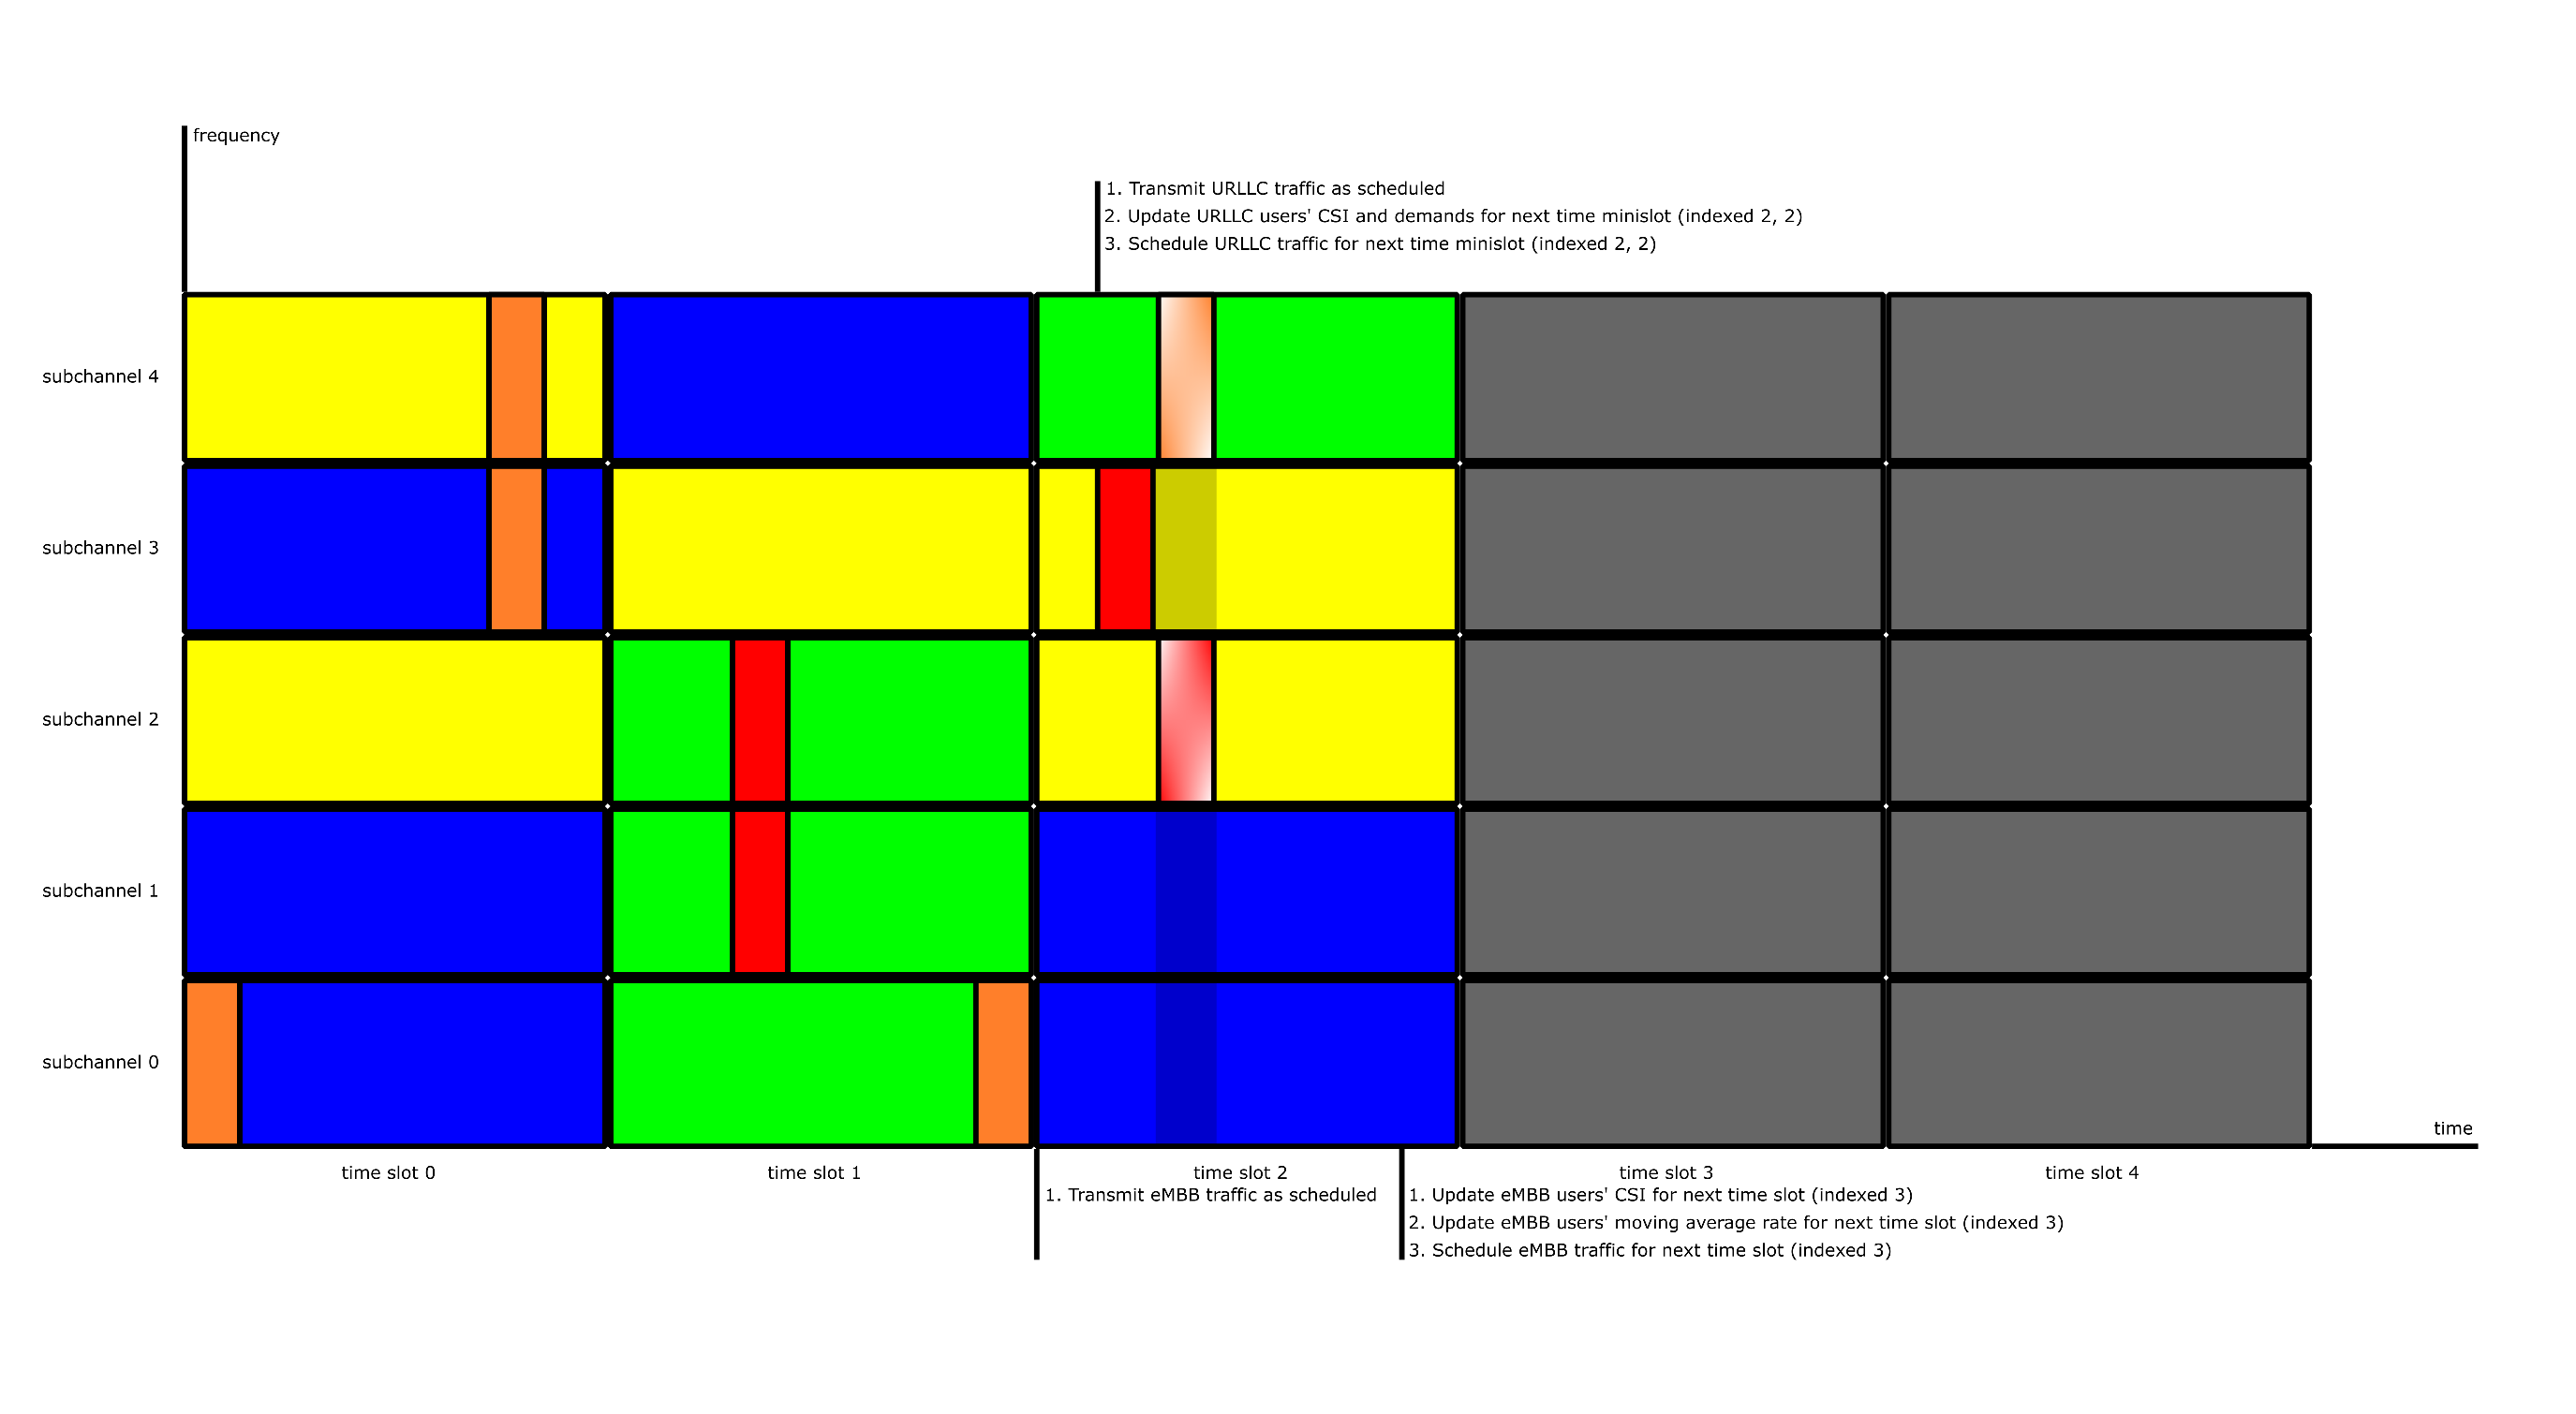
\includegraphics[width=0.8\textwidth]{system_framework}
      \caption{System framework}
    \end{figure}
  \end{itemize}
\end{frame}

\section{Channel Model}
\begin{frame}
  \frametitle{Channel Model}
  \begin{itemize}
    \item Path loss
    \item Shadowing
    \item Thermal noise
    \item Co-channel interference
    \item Channel fading
    \item Inter-symbol interference (ISI)
  \end{itemize}
\end{frame}

\subsection{Path Loss and Shadowing}
\begin{frame}
  \frametitle{Path Loss and Shadowing}
  \begin{itemize}
    \item Subchannel frequency
      \begin{equation}
        \freq{\subchannel} = \freq{0} + \subchannel \frac{ \subchannelBandwidth }{ 10^{ 9 } } \unit{GHz},\quad \forall\subchannel
      \end{equation}
    \item 3D distance
      \begin{align*}
        \embbDist{\embbUser}{\timeSlot} &= \sqrt{ \left( \embbX{\embbUser}{\timeSlot} - \bsX \right)^2 + \left( \embbY{\embbUser}{\timeSlot} - \bsY \right)^2 + \left( \embbZ{\embbUser}{\timeSlot} - \bsZ \right)^2 } &\unit{m},\\
        &\forall\embbUser, \forall\timeSlot\\
        \urllcDist{\urllcUser}{\timeSlot}{\timeMinislot} &= \sqrt{ \left( \urllcX{\urllcUser}{\timeSlot}{\timeMinislot} - \bsX \right)^2 + \left( \urllcY{\urllcUser}{\timeSlot}{\timeMinislot} - \bsY \right)^2 + \left( \urllcZ{\urllcUser}{\timeSlot}{\timeMinislot} - \bsZ \right)^2 } &\unit{m},\\
        &\forall\urllcUser, \forall\timeSlot, \forall\timeMinislot
      \end{align*}
  \end{itemize}
\end{frame}

\begin{frame}
  \begin{itemize}
    \item Path loss and shadowing -- close-in (CI) free space reference distance model
      \begin{equation}
        \plsFunc{\freque}{\distance} = 20 \log_{ 10 }{ \frac{ 4 \pi \freque }{ \lightSpeed } } + 10 \pathLossExponent \log_{ 10 }{ \distance } + \shadowingStddv
      \end{equation}
    \item Path loss exponent and shadowing standard deviation for urban macro-cellular (UMa) line-of-sight (LoS) over frequency and 3D distance ranging from 2 to 73.5GHz and 58 to 930m are derived via minimum mean square error (MMSE) fit by \cite{SRRTGKRKPJ16}
      \begin{align}
        \pathLossExponent &= 2\\
        \shadowingStddv &= 4.6 \unit{dB}
      \end{align}
  \end{itemize}
\end{frame}

\begin{frame}
  \begin{itemize}
    \item Path loss and shadowing
      \begin{align}
        \embbPls{\embbUser}{\timeSlot}{\subchannel} &= \plsFunc{ \freq{\subchannel} }{ \embbDist{\embbUser}{\timeSlot} } &\unit{dB},\quad &\forall\embbUser, \forall\timeSlot, \forall\subchannel\\
        \urllcPls{\urllcUser}{\timeSlot}{\timeMinislot}{\subchannel} &= \plsFunc{ \freq{\subchannel} }{ \urllcDist{\urllcUser}{\timeSlot}{\timeMinislot} } &\unit{dB},\quad &\forall\urllcUser, \forall\timeSlot, \forall\timeMinislot, \forall\subchannel
      \end{align}
    \item Received power -- path loss and shadowing model
      \begin{align}
        \embbPow{\embbUser}{\timeSlot}{\subchannel} &= \txPow - \embbPls{\embbUser}{\timeSlot}{\subchannel} &\unit{dB},\quad &\forall\embbUser, \forall\timeSlot, \forall\subchannel\\
        \urllcPow{\urllcUser}{\timeSlot}{\timeMinislot}{\subchannel} &= \txPow - \urllcPls{\urllcUser}{\timeSlot}{\timeMinislot}{\subchannel} &\unit{dB},\quad &\forall\urllcUser, \forall\timeSlot, \forall\timeMinislot, \forall\subchannel
      \end{align}
  \end{itemize}
\end{frame}

\subsection{Thermal Noise and Co-channel Interference}
\begin{frame}
  \frametitle{Thermal Noise and Co-channel Interference}
  \begin{itemize}
    \item Subchannel thermal noise
      \begin{align}
        \subchannelThermalNoise &= 10^{ \frac{ \thermalNoiseDensity }{ 10 } } \subchannelBandwidth &\unit{W}\\
        &= 10^{ \frac{ -204 }{ 10 } } \cdot 7.2 \cdot 10^{ 5 } &\unit{W}\\
        &\approx -145 &\unit{dB}
      \end{align}
    \item Co-channel interference does not exist in this system model.
  \end{itemize}
\end{frame}

\begin{frame}
  \begin{itemize}
    \item Shannon-Hartley theorem
      \begin{align*}
        \pRateSlot{\embbUser}{\timeSlot}{\subchannel} &= \subchannelBandwidth \log_{ 2 }{ \left( 1 + 10^{ \frac{ \embbPow{\embbUser}{\timeSlot}{\subchannel} - \subchannelThermalNoise }{ 10 } } \right) } \timeSlotDuration \unit{\frac{ bits }{ slot }},\quad\\
        &\forall\embbUser, \forall\timeSlot, \forall\subchannel\\
        \pRateMinislot{\urllcUser}{\timeSlot}{\timeMinislot}{\subchannel} &= \subchannelBandwidth \log_{ 2 }{ \left( 1 + 10^{ \frac{ \urllcPow{\urllcUser}{\timeSlot}{\timeMinislot}{\subchannel} - \subchannelThermalNoise }{ 10 } } \right) } \timeMinislotDuration \unit{\frac{ bits }{ minislot }},\quad\\
        &\forall\urllcUser, \forall\timeSlot, \forall\timeMinislot, \forall\subchannel
      \end{align*}
  \end{itemize}
\end{frame}

\subsection{Channel Fading and ISI}
\begin{frame}
  \frametitle{Channel Fading and ISI}
  \begin{itemize}
    \item Channel fading is resolved by OFDM's cyclic prefix.
    \item ISI is resolved by OFDM's multi-carrier and cylic prefix.
      \begin{itemize}
        \item Multi-carrier has relatively long symbol duration compared to single-carrier transmitting same number of symbols over same frequency bandwidth during same time duration.
        \item Cyclic prefix also serves as inter-symbol guard duration.
      \end{itemize}
    \item Note on resolving ISI using equalization:
      \begin{itemize}
        \item Channel gain is first measured as received signal of a unit impulse transmission, and then used with received signal to decode transmitted signal (I do not understand how this is done).
        \item OFDM performs equalization in frequency domain (I do not understand how this is done).
      \end{itemize}
  \end{itemize}
\end{frame}

\section{Problem}
\begin{frame}
  \frametitle{Offline URLLC Puncturing}
  \begin{itemize}
    \item The system maximizes eMBB traffic's total average rate and fairness \eqref{po:offline}.
    \item For each time slot, the system allocates at most one eMBB user to each subchannel \eqref{pc:offline1}.
    \item For each time slot, the system either schedules or un-schedules a subchannel to each eMBB user \eqref{pc:offline2}.
    \item For each time minislot, the system allocates at most one URLLC user to each subchannel. Also, it schedules $\subchannel^{th}$ subchannel from $\embbUser^{th}$ eMBB user to a URLLC user only if it schedules the subchannel to the eMBB user \eqref{pc:offline3}.
    \item For each time minislot, the system serves URLLC demands without delay \eqref{pc:offline4}.
    \item For each time minislot, the system employs URLLC puncturing instead of superposition \eqref{pc:offline5}.
  \end{itemize}
\end{frame}

\begin{frame}
  \begin{maxi!}
    { \embbVec, \urllcVec }{ \sum_{ \embbUser }{ \utilComp{\avgRate{\embbUser} } } \label{po:offline} }
    {}{}
    \addConstraint
      { \sum_{ \embbUser }{ \embbThree{\embbUser}{\timeSlot}{\subchannel} } }
      { \leq 1,\quad \label{pc:offline1} }
      { \forall\timeSlot, \forall\subchannel }
    \addConstraint
      { \embbThree{\embbUser}{\timeSlot}{\subchannel} }
      { \in \set{ 0, 1 },\quad \label{pc:offline2} }
      { \forall\embbUser, \forall\timeSlot, \forall\subchannel }
    \addConstraint
      { \sum_{ \urllcUser }{\urllcFive{\urllcUser}{\embbUser}{\timeSlot}{\timeMinislot}{\subchannel} } }
      { \leq \embbThree{\embbUser}{\timeSlot}{\subchannel},\quad \label{pc:offline3} }
      { \forall\embbUser, \forall\timeSlot, \forall\timeMinislot, \forall\subchannel }
    \addConstraint
      { \rateMinislot{\urllcUser}{\timeSlot}{\timeMinislot} }
      { \geq \dRateThree{\urllcUser}{\timeSlot}{\timeMinislot},\quad \label{pc:offline4} }
      { \forall\urllcUser, \forall\timeSlot, \forall\timeMinislot }
    \addConstraint
      { \urllcFive{\urllcUser}{\embbUser}{\timeSlot}{\timeMinislot}{\subchannel} }
      { \in \set{ 0, 1 },\quad \label{pc:offline5} }
      { \forall\urllcUser, \forall\embbUser, \forall\timeSlot, \forall\timeMinislot, \forall\subchannel }
  \end{maxi!}
\end{frame}

\begin{frame}
  where
  \begin{align}
    \avgRate{\embbUser} &= \frac{ 1 }{ \timeSlotNum } \sum_{ \timeSlot, \timeMinislot, \subchannel }{ \left( \embbThree{\embbUser}{\timeSlot}{\subchannel} - \sum_{ \urllcUser }{ \urllcFive{\urllcUser}{\embbUser}{\timeSlot}{\timeMinislot}{\subchannel} } \right) \frac{ \pRateSlot{\embbUser}{\timeSlot}{\subchannel} }{ \timeMinislotNum } } &\unit{\frac{ bits }{ slot }}, \label{eq:subchannel}\\
    &\forall\embbUser\\
    \rateMinislot{\urllcUser}{\timeSlot}{\timeMinislot} &= \sum_{ \embbUser, \subchannel }{ \urllcFive{\urllcUser}{\embbUser}{\timeSlot}{\timeMinislot}{\subchannel} \pRateMinislotMin{\urllcUser}{\timeSlot}{\timeMinislot} } &\unit{\frac{ bits }{ minislot }},\\
    &\forall\urllcUser, \forall\timeSlot, \forall\timeMinislot\\
    \pRateMinislotMin{\urllcUser}{\timeSlot}{\timeMinislot} &= \min_{ \subchannel }{ \left\{ \pRateMinislot{\urllcUser}{\timeSlot}{\timeMinislot}{\subchannel} \right\} } &\unit{\frac{ bits }{ minislot }}\\
    &\forall\urllcUser, \forall\timeSlot, \forall\timeMinislot
  \end{align}
\end{frame}

\subsection{Offline eMBB}
\begin{frame}
  \frametitle{Offline Multiplexing URLLC Puncturing -- eMBB}
  \begin{itemize}
    \item Schedule eMBB traffic using \textcolor{red}{only} eMBB channel state information (CSI)
      \begin{maxi!}
        { \embbVec }{ \sum_{ \embbUser }{ \utilComp{\avgRate{\embbUser} } } }
        { \label{pb:embb} }{}
        \addConstraint
          { \sum_{ \embbUser }{ \embbThree{\embbUser}{\timeSlot}{\subchannel} } }
          { \leq 1,\quad }
          { \forall\timeSlot, \forall\subchannel }
        \addConstraint
          { \embbThree{\embbUser}{\timeSlot}{\subchannel} }
          { \in \set{ 0, 1 },\quad \label{pc:binary} }
          { \forall\embbUser, \forall\timeSlot, \forall\subchannel }
      \end{maxi!}
    \item By first relaxing the binary constraint \eqref{pc:binary} and then employing subgradient method, \textcolor{red}{we should be able to} prove by \cite{S05} and by total unimodularity that proportional fairness (PF) scheduling algorithm gives an asymptotically optimal solution.
  \end{itemize}
\end{frame}

\subsection{Online eMBB}
\begin{frame}
  \frametitle{Online Multiplexing URLLC Puncturing -- eMBB}
  \begin{itemize}
    \item Relax binary constraint 
      \begin{maxi!}
        { \relaxEmbbVec }{ \sum_{ \embbUser }{ \utilComp{\relaxAvgRate{\embbUser} } } }
        {}{}
        \addConstraint
          { \sum_{ \embbUser }{ \relaxEmbbThree{\embbUser}{\timeSlot}{\subchannel} } }
          { \leq 1,\quad \label{pc:relax1} }
          { \forall\timeSlot, \forall\subchannel }
        \addConstraint
          { \relaxEmbbThree{\embbUser}{\timeSlot}{\subchannel} }
          { \geq 0,\quad \label{pc:relax2} }
          { \forall\embbUser, \forall\timeSlot, \forall\subchannel }
      \end{maxi!}
    \item Note that the constraint $\relaxEmbbThree{\embbUser}{\timeSlot}{\subchannel} \leq 1,\quad \forall\embbUser, \forall\timeSlot, \forall\subchannel$ is implied for this problem.
    \item The optimal value of this problem is always greater than the optimal value of problem \eqref{pb:embb} (\textcolor{red}{proof needed}).
  \end{itemize}
\end{frame}

\begin{frame}
  \begin{itemize}
    \item Since the feasible average rate set is convex (\textcolor{red}{proof needed}), \cite{S05} shows that the following scheduling policy is asymptotically optimal: For $\curTimeSlot = 0, 1, \dots, \timeSlotNum - 1$
      \begin{equation}
        \relaxCurEmbbVecOpt{\curTimeSlot} \in \argmax_{ \relaxCurEmbbVec{\curTimeSlot} }{ \set{ \gradient{\utilFunc}{\movAvgRateVec{\curTimeSlot}} \transpose \relaxCurRateSlotVec{\curTimeSlot} \largeSetCondition \eqref{pc:relax1}, \eqref{pc:relax2} } }
      \end{equation}
    \item where
      \begin{align}
        \utilFunc \colon \realNonneg{\embbUserNum} &\longrightarrow \real\\
        \rateVec &\longmapsto \sum_{ \embbUser }{ \utilComp{\rateSlotOne{\embbUser}} }
      \end{align}
  \end{itemize}
\end{frame}

\begin{frame}
  \begin{itemize}
    \item For $\curTimeSlot = 0, 1, \dots, \timeSlotNum - 1$
      \begin{maxi!}
        { \relaxCurEmbbVec{\curTimeSlot} }{ \sum_{ \embbUser }{ \frac{ 1 }{ \relaxMovAvgRateTwo{\embbUser}{\curTimeSlot} } \relaxRateSlotTwo{\embbUser}{\curTimeSlot} } }
        { \label{pb:lp} }{}
        \addConstraint
          { \sum_{ \embbUser }{ \relaxEmbbThree{\embbUser}{\curTimeSlot}{\subchannel} } }
          { \leq 1,\quad }
          { \forall\subchannel }
        \addConstraint
          { \relaxEmbbThree{\embbUser}{\curTimeSlot}{\subchannel} }
          { \geq 0,\quad }
          { \forall\embbUser, \forall\subchannel }
      \end{maxi!}
    \item where
      \begin{align}
        \relaxMovAvgRateTwo{\embbUser}{\curTimeSlot} &=
        \begin{cases}
          1 &\curTimeSlot = 0\\
          \left( 1 - \weight \right) \relaxMovAvgRateTwo{\embbUser}{\curTimeSlot - 1} + \weight \relaxRateSlotTwo{\embbUser}{\curTimeSlot - 1} &\otherwise
        \end{cases},\unit{\frac{ bits }{ slot }} \quad \forall\embbUser\\
        \weight &= 0.1
      \end{align}
  \end{itemize}
\end{frame}

\begin{frame}
  \begin{itemize}
    \item Since linear program \eqref{pb:lp} is totally unimodular (\textcolor{red}{proof needed}), it has binary solution(s).
    \item Combining the above statements, binary solution(s) of problem \eqref{pb:lp} gives asymtotically maximum objective value for problem \eqref{pb:embb} (\textcolor{red}{proof needed}).
    \item Also, do notice that the PF scheduling algorithm optimizes problem \eqref{pb:lp}\footnote{Example}.
  \end{itemize}
\end{frame}

\subsection{Online URLLC}
\begin{frame}
  \frametitle{Online Multiplexing URLLC Puncturing -- URLLC}
  \begin{itemize}
    \item For $\curTimeMinislot = 0, 1, \dots, \timeMinislotNum - 1$ in $\curTimeSlot = 0, 1, \dots, \timeSlotNum - 1$
      \begin{maxi!}
        { \curUrllcVec{\curTimeSlot}{\curTimeMinislot} }{ \sum_{ \embbUser }{ \utilComp{\movModAvgRate{\embbUser}{\curTimeSlot}{\curTimeMinislot}} } }
        {}{}
        \constraintOne
        \addConstraint
          { \textcolor{red}{\sum_{ \subchannel }{ \urllcOldFour{\urllcUser}{\curTimeSlot}{\curTimeMinislot}{\subchannel} }} }
          { \textcolor{red}{= \demandSubchannel{\urllcUser}{\curTimeSlot}{\curTimeMinislot},\quad} \label{pc:fix} }
          { \textcolor{red}{\forall\urllcUser} }
        \addConstraint
          { \urllcOldFour{\urllcUser}{\curTimeSlot}{\curTimeMinislot}{\subchannel} }
          { \in \set{ 0, 1 },\quad }
          { \forall\urllcUser, \forall\subchannel }
      \end{maxi!}
    \item where
      \begin{equation}
        \movModAvgRate{\embbUser}{\curTimeSlot}{\curTimeMinislot} = \left( 1 - \weight \right) \movAvgRateMinislot{\embbUser}{\curTimeSlot - 1} + \weight \modRateMinislot{\embbUser}{\curTimeSlot}{\curTimeMinislot} \unit{\frac{ bits }{ minislot }},\quad \forall\embbUser
      \end{equation}
  \end{itemize}
\end{frame}

\begin{frame}
  \begin{itemize}
    \item \textcolor{red}{Punctured} eMBB moving average \textcolor{red}{minislot} rate
      \begin{align}
        \movAvgRateMinislot{\embbUser}{\curTimeSlot - 1} &=
        \begin{cases}
          0 &\curTimeSlot = 0\\
          \frac{ 1 }{ \timeMinislotNum } &\curTimeSlot = 1\\
          \left( 1 - \weight \right) \movAvgRateMinislot{\embbUser}{\curTimeSlot - 2} + \weight \frac{ \rateSlotTwo{\embbUser}{\curTimeSlot - 2} }{ \timeMinislotNum } &\otherwise
        \end{cases}\\
        &\unit{\frac{ bits }{ minislot }},\quad \forall\embbUser
      \end{align}
  \end{itemize}
\end{frame}

\begin{frame}
  \begin{itemize}
    \item Modified eMBB `peak' minislot rate
      \begin{align}
        \modPeakRateMinislot{\embbUser}{\curTimeSlot}{\curTimeMinislot} &=
        \begin{cases}
          \frac{ \relaxRateSlotTwoOpt{\embbUser}{\curTimeSlot} }{ \timeMinislotNum } &\curTimeMinislot = 0\\
          \modRateMinislot{\embbUser}{\curTimeSlot}{\curTimeMinislot - 1} &\otherwise
        \end{cases}\\
        &\unit{\frac{ bits }{ minislot }},\quad \forall\embbUser
      \end{align}
    \item Modified eMBB minislot rate
      \begin{align}
        \modRateMinislot{\embbUser}{\curTimeSlot}{\curTimeMinislot} &= \left( 1 - \frac{ \sum_{ \subchannel }{ \left( \embbThree{\embbUser}{\curTimeSlot}{\subchannel} \wedge \sum_{ \urllcUser }{ \urllcOldFour{\urllcUser}{\curTimeSlot}{\curTimeMinislot}{\subchannel} } \right) } }{ \sum_{ \subchannel }{ \embbThree{\embbUser}{\curTimeSlot}{\subchannel} } } \right) \modPeakRateMinislot{\embbUser}{\curTimeSlot}{\curTimeMinislot} \label{eq:noSubchannel}\\
        &\unit{\frac{ bits }{ minislot }},\quad \forall\embbUser\\
      \end{align}
  \end{itemize}
\end{frame}

\begin{frame}
  \begin{itemize}
    \item Linearize modified eMBB minislot rate in $\curUrllcVec{\curTimeSlot}{\curTimeMinislot}$\footnote{Example}
      \begin{align}
        \modRateMinislot{\embbUser}{\curTimeSlot}{\curTimeMinislot} &= \left( 1 - \frac{ \inner{ \urllcMat{\curTimeSlot}{\curTimeMinislot}( \colon, col( \embbMat{\embbUser}{\curTimeSlot} ) ) }{ 1 } }{ \sum_{ \subchannel }{ \embbThree{\embbUser}{\curTimeSlot}{\subchannel} } } \right) \modPeakRateMinislot{\embbUser}{\curTimeSlot}{\curTimeMinislot}\\
        &\unit{\frac{ bits }{ minislot }},\quad \forall\embbUser
      \end{align}
  \end{itemize}
\end{frame}

\begin{frame}
  \frametitle{Convex}
  \begin{itemize}
    \item Equivalent program 1
      \begin{maxi!}
        { \curUrllcVec{\curTimeSlot}{\curTimeMinislot} }{ \sum_{ \embbUser }{ \utilComp{\movModAvgRate{\embbUser}{\curTimeSlot}{\curTimeMinislot}} } }
        {}{}
        \constraintOne
        \constraintTwo
        \addConstraint
          { \binaryFunc }
          { = 0,\quad }
          { \forall\urllcUser, \forall\subchannel }
      \end{maxi!}
  \end{itemize}
\end{frame}

\begin{frame}
  \frametitle{Convex (Continued)}
  \begin{itemize}
    \item Equivalent program 2
      \begin{maxi!}
        { \curUrllcVec{\curTimeSlot}{\curTimeMinislot} }{ \sum_{ \embbUser }{ \utilComp{\movModAvgRate{\embbUser}{\curTimeSlot}{\curTimeMinislot}} } }
        {}{}
        \constraintOne
        \constraintTwo
        \addConstraint
          { \binaryFunc }
          { \geq 0,\quad }
          { \forall\urllcUser, \forall\subchannel }
        \addConstraint
          { \sum_{ \urllcUser, \subchannel }{ \binaryFunc } }
          { = 0 }
          {}
      \end{maxi!}
  \end{itemize}
\end{frame}

\begin{frame}
  \frametitle{Convex (Continued)}
  \begin{itemize}
    \item Equivalent program 3
      \begin{maxi!}
        { \curUrllcVec{\curTimeSlot}{\curTimeMinislot} }{ \sum_{ \embbUser }{ \utilComp{\movModAvgRate{\embbUser}{\curTimeSlot}{\curTimeMinislot}} } }
        {}{}
        \constraintOne
        \constraintTwo
        \addConstraint
          { \urllcOldFour{\urllcUser}{\curTimeSlot}{\curTimeMinislot}{\subchannel} }
          { \geq 0,\quad }
          { \forall\urllcUser, \forall\subchannel }
        \addConstraint
          { \sum_{ \urllcUser, \subchannel }{ \binaryFunc } }
          { = 0 }
          {}
      \end{maxi!}
  \end{itemize}
\end{frame}

\begin{frame}
  \frametitle{Convex (Continued)}
  \begin{itemize}
    \item Equivalent program 4
      \begin{mini!}
        { \curUrllcVec{\curTimeSlot}{\curTimeMinislot} }{ -\sum_{ \embbUser }{ \utilComp{\movModAvgRate{\embbUser}{\curTimeSlot}{\curTimeMinislot}} } }
        {}{}
        \constraintOne
        \constraintTwo
        \addConstraint
          { \urllcOldFour{\urllcUser}{\curTimeSlot}{\curTimeMinislot}{\subchannel} }
          { \geq 0,\quad }
          { \forall\urllcUser, \forall\subchannel }
        \addConstraint
          { \sum_{ \urllcUser, \subchannel }{ \binaryFunc } }
          { = 0 }
          {}
      \end{mini!}
  \end{itemize}
\end{frame}

\begin{frame}
  \frametitle{Convex (Continued)}
  \begin{itemize}
    \item Polyhedron
      \begin{equation}
        \polyhedron = \left\{ \curUrllcVec{\curTimeSlot}{\curTimeMinislot} \largeSetCondition
          \begin{aligned}
            &\sum_{ \urllcUser }{ \urllcOldFour{\urllcUser}{\curTimeSlot}{\curTimeMinislot}{\subchannel} } &\leq 1\\
            &\sum_{ \subchannel }{ \urllcOldFour{\urllcUser}{\curTimeSlot}{\curTimeMinislot}{\subchannel} } &= \demandSubchannel{\urllcUser}{\curTimeSlot}{\curTimeMinislot}\\
            &\urllcOldFour{\urllcUser}{\curTimeSlot}{\curTimeMinislot}{\subchannel} &\geq 0
          \end{aligned} \right\}
      \end{equation}
 \end{itemize}
\end{frame}

\begin{frame}
  \frametitle{Convex (Continued)}
  \begin{itemize}
    \item Equivalent program 5
      \begin{mini!}
        { \curUrllcVec{\curTimeSlot}{\curTimeMinislot} }{ -\sum_{ \embbUser }{ \utilComp{\movModAvgRate{\embbUser}{\curTimeSlot}{\curTimeMinislot}} } }
        { \label{pb:equi5} }{}
        \addConstraint
          { \curUrllcVec{\curTimeSlot}{\curTimeMinislot} }
          { \in \polyhedron }
          {}
        \addConstraint
          { \sum_{ \urllcUser, \subchannel }{ \binaryFunc } }
          { = 0 }
          {}
      \end{mini!}
  \end{itemize}
\end{frame}

\begin{frame}
  \frametitle{Convex (Continued)}
  \begin{itemize}
    \item Feasible solution
      \begin{equation}
        \feaSolVec \in \polyhedron \cap \set{ \curUrllcVec{\curTimeSlot}{\curTimeMinislot} \largeSetCondition \sum_{ \urllcUser, \subchannel }{ \binaryFunc } = 0 }
      \end{equation}
  \end{itemize}
\end{frame}

\begin{frame}
  \frametitle{Convex (Continued)}
  \begin{itemize}
    \item Penalized program
      \begin{mini!}
        { \curUrllcVec{\curTimeSlot}{\curTimeMinislot} }{ -\sum_{ \embbUser }{ \utilComp{\movModAvgRate{\embbUser}{\curTimeSlot}{\curTimeMinislot}} } + \penaltyMultiplier \sum_{ \urllcUser, \subchannel }{ \binaryFunc } }
        { \label{pb:penalized} }{}
        \addConstraint
          { \curUrllcVec{\curTimeSlot}{\curTimeMinislot} }
          { \in \polyhedron }
          {}
        \addConstraint
          { \sum_{ \urllcUser, \subchannel }{ \binaryFunc } }
          { \textcolor{red}{\geq} 0 }
          {}
      \end{mini!}
    \item where \scalebox{0.6}{$\penaltyMultiplier > \frac{ \left( -\sum_{ \embbUser }{ \utilComp{\movModAvgRate{\embbUser}{\curTimeSlot}{\curTimeMinislot}} } \right)^{\text{at } \feaSolVec} - \inf_{ \curUrllcVec{\curTimeSlot}{\curTimeMinislot} }{ \set{ -\sum_{\embbUser}{ \utilComp{\movModAvgRate{\embbUser}{\curTimeSlot}{\curTimeMinislot}} } \vert \curUrllcVec{\curTimeSlot}{\curTimeMinislot} \in \polyhedron, \sum_{ \urllcUser, \subchannel }{ \binaryFunc } \geq 0 } } }{ \inf_{ \curUrllcVec{\curTimeSlot}{\curTimeMinislot} }{ \set{ \sum_{ \urllcUser, \subchannel }{ \binaryFunc } \vert \curUrllcVec{\curTimeSlot}{\curTimeMinislot} \in vertices(\polyhedron), \sum_{ \urllcUser, \subchannel }{ \binaryFunc } > 0 } } } \geq 0$}
    \item In practice, $\penaltyMultiplier$ is set to a very large number.
  \end{itemize}
\end{frame}

\begin{frame}
  \frametitle{Convex (Continued)}
  \begin{block}{Theorem 1 \cite{LPN12}}
    If $-\sum_{ \embbUser }{ \utilComp{\movModAvgRate{\embbUser}{\curTimeSlot}{\curTimeMinislot}} }$ and $\sum_{ \urllcUser, \subchannel }{ \binaryFunc }$ are concave in $\curUrllcVec{\curTimeSlot}{\curTimeMinislot}$, then problem \eqref{pb:equi5} and \eqref{pb:penalized} are equivalent.
  \end{block}
\end{frame}

\begin{frame}
  \frametitle{Convex (Continued)}
  \begin{itemize}
    \item `Equivalent' program 6
      \begin{mini*}
        { \curUrllcVec{\curTimeSlot}{\curTimeMinislot} }{ -\sum_{ \embbUser }{ \utilComp{\movModAvgRate{\embbUser}{\curTimeSlot}{\curTimeMinislot}} } + \penaltyMultiplier \sum_{ \urllcUser, \subchannel }{ \binaryFunc } }
        {}{}
        \constraintOne
        \constraintTwo
        \addConstraint
          { \urllcOldFour{\urllcUser}{\curTimeSlot}{\curTimeMinislot}{\subchannel} }
          { \geq 0,\quad }
          { \forall\urllcUser, \forall\subchannel }
        \addConstraint
          { \sum_{ \urllcUser, \subchannel }{ \binaryFunc } }
          { \geq 0 }
          {}
      \end{mini*}
  \end{itemize}
\end{frame}

\begin{frame}
  \frametitle{Convex (Continued)}
  \begin{itemize}
    \item `Equivalent' program 7
      \begin{mini!}
        { \curUrllcVec{\curTimeSlot}{\curTimeMinislot} }{ -\sum_{ \embbUser }{ \utilComp{\movModAvgRate{\embbUser}{\curTimeSlot}{\curTimeMinislot}} } + \penaltyMultiplier \sum_{ \urllcUser, \subchannel }{ \binaryFunc } }
        {}{}
        \constraintOne
        \constraintTwo
        \addConstraint
          { \urllcOldFour{\urllcUser}{\curTimeSlot}{\curTimeMinislot}{\subchannel} }
          { \geq 0,\quad }
          { \forall\urllcUser, \forall\subchannel }
      \end{mini!}
  \end{itemize}
\end{frame}

\begin{frame}
  \frametitle{Convex (Continued)}
  \begin{itemize}
    \item Define
      \begin{equation}
        \concaveBinary{\curUrllcVec{\curTimeSlot}{\curTimeMinislot}} = \sum_{ \urllcUser, \subchannel }{ \binaryFunc }
      \end{equation}
    \item Since $\concaveBinaryFunc$ is a differentiable concave function
      \begin{align}
        \concaveBinary{\curUrllcVec{\curTimeSlot}{\curTimeMinislot}} &\leq \concaveBinary{\feaSolVec} + \gradient{\concaveBinaryFunc}{\feaSolVec} \transpose \left( \curUrllcVec{\curTimeSlot}{\curTimeMinislot} - \feaSolVec \right)\\
        &= \sum_{ \urllcUser, \subchannel }{ \feaSol{\urllcUser}{\subchannel} \left( 1 - \feaSol{\urllcUser}{\subchannel} \right) } + \sum_{ \urllcUser, \subchannel }{ \left( 1 - 2 \feaSol{\urllcUser}{\subchannel} \right) \left( \urllcOldFour{\urllcUser}{\curTimeSlot}{\curTimeMinislot}{\subchannel} - \feaSol{\urllcUser}{\subchannel} \right) }\\
        &= approx(\curUrllcVec{\curTimeSlot}{\curTimeMinislot})
      \end{align}
  \end{itemize}
\end{frame}

\begin{frame}
  \frametitle{Convex (Continued)}
   \begin{itemize}
    \item Subroutine solving difference of convex (DC) programming
      \begin{mini!}
        { \curUrllcVec{\curTimeSlot}{\curTimeMinislot} }{ -\sum_{ \embbUser }{ \utilComp{\movModAvgRate{\embbUser}{\curTimeSlot}{\curTimeMinislot}} } + \penaltyMultiplier approx(\curUrllcVec{\curTimeSlot}{\curTimeMinislot}) }
        {}{}
        \constraintOne
        \constraintTwo
        \addConstraint
          { \urllcOldFour{\urllcUser}{\curTimeSlot}{\curTimeMinislot}{\subchannel} }
          { \geq 0,\quad }
          { \forall\urllcUser, \forall\subchannel }
      \end{mini!}
  \end{itemize}
\end{frame}

\begin{frame}
  \frametitle{Greedy}
  \begin{itemize}
    \item The idea is to puncture `wealthies' eMBB users in the current time slot\footnote{Example}.
  \end{itemize}
\end{frame}

\section{Issues}
\begin{frame}
  \frametitle{Issues}
  \begin{itemize}
    \item Due to missing of constraint \eqref{pc:fix}, the obvious optimal solution of the convex method is to not allocate any subchannels to URLLC users.
    \item It is then questionable why greedy method can perform as good as convex one.
      \begin{figure}
        \includegraphics[width=0.4\textwidth]{experiment}
        \caption{Experiment result}
      \end{figure}
  \end{itemize}
\end{frame}

\begin{frame}
  \frametitle{Issues -- Convex}
  \begin{itemize}
    \item Since $-\sum_{ \embbUser }{ \utilComp{\movModAvgRate{\embbUser}{\curTimeSlot}{\curTimeMinislot}} }$ is not concave in $\curUrllcVec{\curTimeSlot}{\curTimeMinislot}$, theorem 1 is not applicable, and hence the penalized program's optimality is questionable\footnote{Example}.
    \item Even if we assume the penalized program's optimality, the subroutine solving it does not have optimality bounds (in single cell case, my algorithm is optimal).
    \item There is no theory backing up their objective function for URLLC's online multiplexing problem (my model possesses analytical justification).
  \end{itemize}
\end{frame}

\begin{frame}
  \frametitle{Issues -- Greedy}
  \begin{itemize}
    \item In greedy algorithm, unlike PF, eMBB subchannel-wise rates are not considered when puncturing \eqref{eq:noSubchannel} (do note that my model does take this into account \eqref{eq:subchannel}).
    \item In greedy algorithm, moving average rate employs outdated information (fixing this is straightforward).
    \item Greedy algorithm does not have optimality bounds (in multicell case, my algorithm has a guaranteed approximation ratio).
  \end{itemize}
\end{frame}

\begin{frame}
  \frametitle{Contributions}
  \begin{itemize}
    \item Based on the existing eMBB scheduler, a model for joint scheduling of punctured eMBB and URLLC traffic as an optimization problem that maximizes the eventual aggregate utility of the eMBB users subject to latency constraints for the URLLC users.
    \item Model for the delay and reliability of URLLC traffic from a media access control (MAC) layer perspective.
    \item Two new resource allocation algorithms to align with practical implementation for downlink scheduling in the 5G system.
  \end{itemize}
\end{frame}

\begin{frame}
  \frametitle{References}
  \printbibliography[heading=none]
\end{frame}

\end{document}
